\usepackage[ngerman, english]{babel}


\title{Goal Setting Workshop}
\author{Felix Karg}


\graphicspath{ {./img/} {../template/} {../template_tex/} } % add further graphics paths here

\newif\iftwocols
% \twocolsfalse
\twocolstrue


\usepackage{etex}
\usepackage{graphicx}
\usepackage[export]{adjustbox}
\usepackage{multicol}
\usepackage{pdfpcnotes}
\usepackage{pdfpages}
% \usepackage[dvipsnames]{xcolor}


% \usepackage{minted}
% \usemintedstyle{pastie}


\usetheme[numbering=fraction, progressbar=frametitle]{metropolis}


\date{December 29, 2020}
% \date{12. Juli 2019}


% \institute{Add Your Institute here}
% \titlegraphic{\vspace{4cm} \hspace{7cm} \includegraphics[height=2cm]{Logo_INST}}
% \titlegraphic{\vspace{4cm} \hspace{7cm} \Huge\LaTeX}

\iftwocols
\AtBeginSection[]
{
    \large
    \begin{frame}{Agenda}
        \begin{multicols}{2}
            \tableofcontents[currentsection]
        \end{multicols}
        \clearpage
    \end{frame}
}

\AtBeginSubsection[]
{
    \large
    \begin{frame}{Agenda}
        \begin{multicols}{2}
            \tableofcontents[currentsection,currentsubsection]
        \end{multicols}
        \clearpage
    \end{frame}
}

\else

\AtBeginSection[]
{
    \large
    \begin{frame}{Agenda}
        \tableofcontents[currentsection]
        \clearpage
    \end{frame}
}

\AtBeginSubsection[]
{
    \large
    \begin{frame}{Agenda}
        \tableofcontents[currentsection,currentsubsection]
        \clearpage
    \end{frame}
}
\fi


\begin{document}

\maketitle

% multicols from:
% https://tex.stackexchange.com/questions/24343/splitting-toc-into-two-columns-on-single-frame-in-beamer

%%%%%%%%%%%%%%%%%%%%%%%%%%%%%%%%%%%%%%%%%%%%%%%%%%%%%%%%%%%%%%%%%%%%%%%%%%%%%%%%%%%%%%%%%%%%%%%%%%%%%%%%%%%%%%%%%%%

\iftwocols
\begin{frame}{Agenda}
    \large
    \begin{multicols}{2}
%        \tableofcontents[hidesubsections]
        \tableofcontents[]
    \end{multicols}
    % \clearpage
\end{frame}

\else

\begin{frame}{Agenda}
    \large
%   \tableofcontents[hidesubsections]
    \tableofcontents[]
    % \clearpage
\end{frame}
\fi


\newcommand{\code}[1]{
    \begin{center}
    \setlength{\fboxrule}{1pt}
    \setlength{\fboxsep}{8pt}
        {\fbox{\parbox{0.81\textwidth}{#1}}}
   \end{center}
}

\newenvironment{codeboxed}[1]
        {\begin{minipage}{\linewidth}\begin{center}#1\\[1ex]\begin{tabular}{|p{\textwidth}|}\hline}
        {\\\hline\end{tabular}\end{center}\end{minipage}}


\newcommand{\backupbegin}{
   \newcounter{finalframe}
   \setcounter{finalframe}{\value{framenumber}}
}

\newcommand{\backupend}{
   \setcounter{framenumber}{\value{finalframe}}
}


\newcommand{\mailto}[1]{
    \href{mailto:#1}{#1}
}

\newcommand{\todo}[1]{
    {\Large\color{red}{(TODO: #1)}}
}

% \definecolor{green1}{RGB}{38, 69, 37} % #264525
\definecolor{green1}{RGB}{72, 129, 69} % #488145
% \definecolor{blue1}{RGB}{7, 43, 94} % #072b5e
\definecolor{blue1}{RGB}{14, 82, 179} % #0e52b3
% \definecolor{violet1}{RGB}{58, 38, 68} % #3a2644
\definecolor{violet1}{RGB}{108, 72, 126} % #6c487e
% \definecolor{orang1}{RGB}{, , 0} % #663400
\definecolor{orang1}{RGB}{193, 98, 0} % #c16200


\newcommand{\green}[1]{
    \textcolor{green1}{#1}
}
\newcommand{\blue}[1]{
    \textcolor{blue1}{#1}
}
\newcommand{\vio}[1]{
    \textcolor{violet1}{#1}
}
\newcommand{\orang}[1]{
    \textcolor{orang1}{#1}
}




\newif\ifonline
\onlinefalse
% \onlinefalse
% usage:
% \ifonline
%   <true text>
% \else % <- optional
%   <false text>
% \fi

%%%%%%%%%%%%%%%%%%%%%%%%%%%%%%%%%%%%%%%%%%%%%%%%%%BEGINNING%%%%%%%%%%%%%%%%%%%%%%%%%%%%%%%%%%%%%%%%
\section{Examples}

\begin{frame}[c]
     Here a citation: \cite{benchcpp}
\end{frame}

\begin{frame}[c]{Example slide}
    \Large
    \begin{itemize}[<+->]
        \item First Element
        \item Second Element
        \item Third Element
    \end{itemize}
\end{frame}

\begin{frame}[c]{Other example slide}
    \Large
    \begin{itemize}[<+(1)->]
        \item First Element
        \item Second Element
        \item Third Element
    \end{itemize}
\end{frame}

\begin{frame}[c]{Yet another example slide}
    \Large
    \begin{itemize}
        \item First Element
            \pause
        \item Second Element
            \pause
        \item Third Element
    \end{itemize}
\end{frame}








\section{Jetzt}

\subsection{Einführung}

\begin{frame}[c]{Problem: Zu viel zu tun}
    \large
    \begin{aquote}{David Allen}
        When you're no longer drowning, you can think about which way to
        paddle.
    \end{aquote}
    \pnote{Häufig kommt es einem vor, als ob man untergehen würde}
    \pnote{Also: Erstmal müssen wir schwimmen lernen}
\end{frame}


\begin{frame}[c]{Lösung}
    
\includegraphics[width=0.6\textwidth]{writing} (Bild von \cite{writing-pic}) \\
    \vspace{0.5cm}
    Schritt Eins: \enquote{Jetzt}-Situation erfassen und strukturieren.
    \pnote{Alles was noch unsere Aufmerksamkeit brauchen wird, aufschreiben}
\end{frame}


\subsection{Unerledigtes}

\begin{frame}[c]{Definition: Unerledigtes}
    \begin{itemize}[<+(1)->]
        \item Antworten, die ausstehen (z.B. Mails)
        \item Angefangene Projekte
        \item Unaufgeräumte Unterhosen
        \item Unbezahlte Steuern (z.B. für Haustiere)
        \item Veranstaltungen, für die man noch etwas vorbereiten muss (z.B. Todos)
        \item Arztbesuche, Reparaturen, Termine
        \item Versprechen, die noch zu erledigen sind
    \end{itemize}
    \pause
    Alles, was noch nicht erledigt ist, oder noch Aufmerksamkeit
    benötigt. Sei konkret, \enquote{Reich werden} zählt nicht.
\end{frame}


\begin{frame}[c]{Hilfsmittel}
    \large
    \begin{itemize}[<+(1)->]
        \item Deine (aktuelle) Todo-Liste (und weitere)
        \item Stift \& Papier (oder anderes Listenerstellungswerkzeug)
        \item GTD Mind Sweep Trigger List \cite{trigger-list} ( \url{https://gettingthingsdone.com/wp-content/uploads/2014/10/Mind_Sweep_Trigger_List.pdf} )
    \end{itemize}
    \pnote{Link schicken}
\end{frame}

\begin{frame}[c]
    \large
    \begin{block}{Aufgabe: Situation erfassen}
    \begin{itemize}
        \item Schreib alles auf, was deine Aufmerksamkeit hat (oder haben sollte!)
        \item Sowohl privat, als auch für's Studium oder die Arbeit!
        \item Erledige alles direkt, was weniger als 2 Minuten braucht!
        \item Ziele kommen auf eine separate Liste!
    \end{itemize}
    \end{block}
    \pnote{Zeit: ~30min}
\end{frame}
\fpause


\subsection{Organisation}

\begin{frame}[c]{Definition: Projekt}
    Ein \blue{Projekt} ist alles, was \textbf{mehr als eine} \green{konkrete
    Aufgabe} benötigt, um abgeschlossen zu werden. \newline \newline \pause
    \textbf{Beispiel:} Wenn man \blue{jemandem ein Geschenk besorgen}
    will, muss man zuerst \green{herausfinden, was die Person mag.}
\end{frame}


\begin{frame}[c]{Definition: Kontext}
    % locations, people
    \orang{Kontext} beschreibt eine \textbf{konkrete Eigenschaft} einer
    \green{Aufgabe} oder einem \blue{Projekt.} Häufig die Abhängigkeit zu einem
    bestimmten \textbf{Ort}, einer \textbf{Umgebung}, oder \textbf{Person}.
    \newline \newline \pause
    \textbf{Beispiele:}
    \begin{itemize}
        \item \orang{Zuhause}, \orang{am PC}
        \item \orang{dauert kurz}, \orang{dauert lang}
        \item \orang{Treffen Mentor}, \orang{Treffen Tobi}
    \end{itemize}
\end{frame}


\begin{frame}[c]{Bemerkungen}
    \large
    Normal ist:
    \begin{itemize}[<+(1)->]
        \item Dir fallen weitere Aufgaben ein, die unerledigt sind ($\rightarrow$ aufschreiben)
        \item Dir fällt auf, dass etwas ein Projekt ist \\ ($\rightarrow$ finde heraus, was die {\em nächste unerledigte Aufgabe} ist)
    \end{itemize}
\end{frame}


\begin{frame}[c]
    \large
    \begin{block}{Aufgabe: Projekte zusammenfassen}
    Fasse thematisch zusammenhängende \green{Aufgaben} zu \blue{Projekten} und
    \orang{Kontexten} zusammen, und markiere zusammengehörende Elemente
    eindeutig (z.B.: Symbol mit einheitlicher Farbe).
    \end{block}
    \pnote{Zeit: 20+ min}
\end{frame}

\fpause


\subsection{Rückblick}

\begin{frame}[c]{Optional: Jahresrückblick}
    \begin{itemize}[<+(1)->]
        \item Zusätzliche, ausführliche Trigger-List
        \item Kann {\em sehr} viel Zeit in Anspruch nehmen
        \item Kann Sinn machen, gleichzeitig Ziele zu sammeln
        \item Ressourcen: \url{https://drive.google.com/file/d/0B2PaeRjVqAN7MngxTXFPQkpLVjg/view} \cite{8760-hours} (Seiten 11-15) (oder anschließend in dieser PDF)
    \end{itemize}
    \pnote{Zeit: 30+ min}
\end{frame}

% \includepdf[pages={11-15},frame,pagecommand={},width=\textwidth]{8760-hours-v2.pdf}
% \includepdf[fitpaper=true,pages=-,frame,pagecommand={},width=\textwidth]{8760-hours-v2.pdf}
{
    \addtocounter{framenumber}{5}
    \setbeamercolor{background canvas}{bg=}
    \includepdf[pages={11-15}]{8760-hours-v2.pdf}
}

\fpause

\section{Ziele}

\subsection{Visualisieren}
% successful
% unsuccessful

% Past Authoring:
% It is difficult to know who you are, where you should go, or how you should
% get there, unless you know where you came from. The Past Authoring Program
% has therefore been designed to help you write a structured autobiography. The
% program will help you:
% - Divide your life into seven different time periods or epochs.
% - Identify the most significant events that occurred during each epoch.
% - Describe how each of those experiences has shaped who you are today.



\begin{frame}[c]
    \begin{block}{Aufgabe: Gutes Visualisieren}
    Stell dir vor, welche:
    \begin{itemize}
        \item Art von Person du sein möchtest
        \item Fähigkeiten (Skills) du erlangt haben möchtest
        \item Beziehungen zu dir selbst, Freunden und Familie, Anderen, du haben möchtest
        \item Freizeitaktivitäten du genießen möchtest
    \end{itemize}
    \pause
    In den nächsten 6 Monaten / 3 Jahren / 5 Jahren?
    \end{block}
    % Future Authoring:
    % specifically describe the type of person they wanted to be, the skills they wanted to attain, and the relationships they wanted to have, among other things
    % You will be asked to consider the people you admire, things you could do better, your educational and career goals, what habits you would like to improve, your family life, your social network, and your leisure activities.
    % timeframes: 6mo/2y/5y

    % source of positive emotion going forward

    % second part: detailed writing out how to do this
\end{frame}


\begin{frame}[c]
    \begin{block}{Aufgabe: Schlechtes Visualisieren}
    % the ways you are radically insufficient and your faults
    % how _you_ would degenerate
    % what is something you don't want to happen in 6mo/2y/5y
    Was passiert, wenn du:
    \begin{itemize}
        \item Deinen schlechten Gewohnheiten nachgibst
        \item Nicht auf deine Gesundheit achtest
        \item Dich von deinen Freunden entfernst
        \item Deine Ziele (wieder) nicht erreichst
    \end{itemize}
    \pause
    In den nächsten 6 Monaten / 3 Jahren / 5 Jahren?
    \end{block}
\end{frame}



% \begin{frame}[c]{Was man erwarten kann}
%     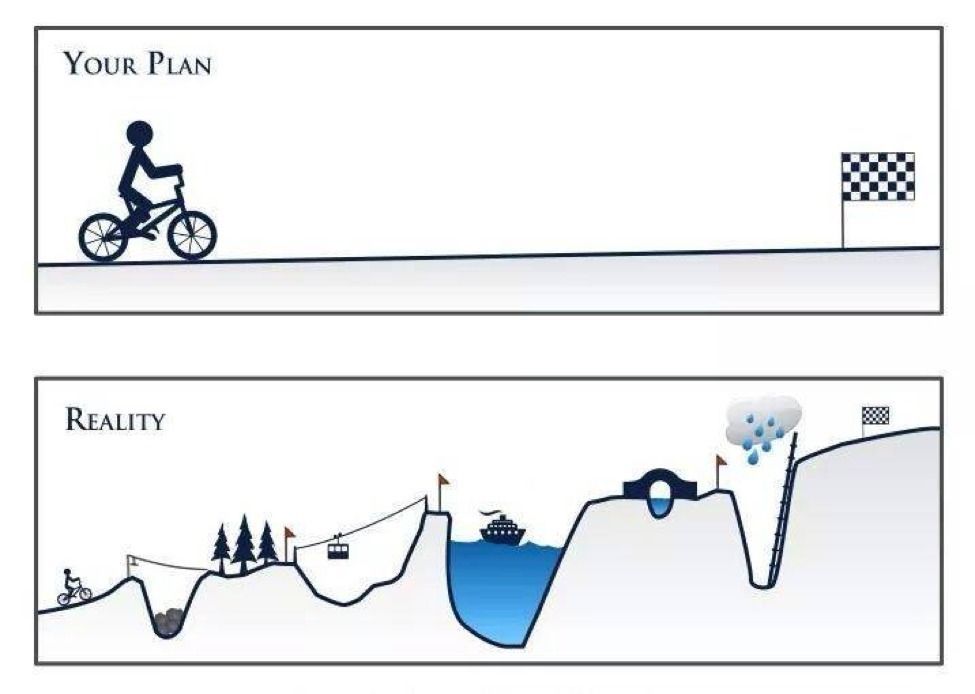
\includegraphics[height=0.8\textheight]{plan-reality} \\
%     Bild von \cite{plan-reality-pic-2}
% \end{frame}



\subsection{Leitmotiv}

\begin{frame}[c]{Warum möchte man ein Leitmotiv haben?}
    \large
    \begin{itemize}[<+(1)->]
        \item Gibt die Richtung freier vor, als konkrete Ziele
        \item Erlaubt schnelleres Wechseln von Zielen
        \item Erlaubt mehr Freiheit zu Experimentieren
        \item Erfolgserlebnis, unabhängig konkreter Pläne
    \end{itemize}
\end{frame}


\addtocounter{framenumber}{-1}
\begin{frame}<handout:1,2>[c]{Definition: Leitmotiv}
    \vspace{0.5cm}
    \large{
    \onslide<handout:1-2>
    Ein Leitmotiv ist:}
    \begin{itemize}[<+(1)->]
        \large
        \item Allgemein
        \item Richtungsweisend
        \item Resonierent
    \end{itemize}
    \pause
    \vspace{0.4cm}
    { \onslide<handout:2>
      \addtocounter{framenumber}{1}
    }
    \onslide<5-|handout:2>{\textbf{Beispiel:} Jahr des ...}
    \begin{multicols}{2}
    \begin{itemize}[<+(1)->]
        \item Lesens
        \item Lernens
        \item Schreibens
        \item Erforschens
    \end{itemize}
    \end{multicols}
\end{frame}



\begin{frame}[c]
    \Large
    \begin{block}{Aufgabe: Leitfaden finden}
    Während des Workshops Aufschreiben, wenn dir etwas in den Sinn kommt!
    \end{block}
\end{frame}


% \begin{frame}[c]{Wie finden}
%     \begin{itemize}[<+(1)->]
%         \item When were you able to use your best talents, skills, and gifts? What were you doing? How did you feel?
%         \item What did you realize you were good at that you didn’t know or claim before now?
%         \item How did you grow? What do you know now that you didn’t know last year?
%         \item What did you do that gave your life meaning? How much time did you spend in that zone?
%         \item When did you avoid doing something uncomfortable even though you now know you should have spoken up or acted?
%         \item What did you put off that you wished you had spent more time on?
%
%     \end{itemize}
% \end{frame}



\subsection{Finden}

\begin{frame}[c]{Ziele Trigger List}
    \footnotesize
    % \begin{multicols}{2}
    \begin{itemize}
        % \item What would excite you, if you had the chance of doing?
        \item Worauf würdest du dich richtig freuen, wenn du die Möglichkeit dazu hättest?
        % \item What would make you fulfilled, if you had done it?
        \item Was würde dich erfüllen, wenn du es getan hättest?
        % \item What do you want to strive for? (e.g. World Peace, Revolutionizing Education, …)
        \item Wonach strebst du? (z.B. Weltfrieden, Kinder in Afrika retten, ...)
        % \item What would you do if there was no way to fail?
        \item Was würdest du tun, wenn du garantiert Erfolg hättest?
        % \item What do you want to have? (This can be material wants, achievements, …)
        \item Was möchtest du haben? (z.B. Materielles, Erfolge, ...)
        % \item What do you want to be? (A great cook, fluent in French, …)
        \item Was wärst du gerne? (z.B. guter Koch, jemand Bewundernswertes, ...)
        % \item What would you do with 100 million in the bank?
        \item Was würdest du mit 100 Millionen auf dem Konto tun?
        % \item Which places would you want to go to?
        \item Was für Orte willst du besuchen?
        % \item What do you want to do before you die?
        \item Was würde auf deiner Bucket-List stehen?
        % \item What did you always want to learn, but never had the time for?
        \item Was wolltest du schon immer lernen?
        \item Was ist etwas, wofür du nie Zeit hattest?
    \end{itemize}
    % \end{multicols}
\end{frame}


\begin{frame}[c]
    \begin{block}{Aufgabe: Ziele aufschreiben}
    Regeln:
    \begin{itemize}
        \item Alles aufschreiben. Sortiert wird später
        \item Egal ob momentan Erreichbar oder nicht
        \item Langsam, Punkt für Punkt durchgehen
        \item Sei Ehrlich!
        \item Träume!
    \end{itemize}
    \end{block}
\end{frame}



\subsection{Reduzieren}

\addtocounter{framenumber}{1}
\begin{frame}[standout]
    \LARGE
    Achtung: Falls du die momentane Liste behalten willst, lohnt es sich, jetzt
    ein Foto oder eine Kopie davon anzulegen, da wir die Ziel-Liste im
    folgenden intensiv bearbeiten werden.
\end{frame}

\begin{frame}[c]{Vorbereitung}
    \Large
    Wandle alle Ziele, in denen du etwas {\em sein} möchtest, in ein Ziel um,
    in dem du etwas {\em tun} möchtest. \newline \newline \pause
    \textbf{Beispiel:} "guter Koch {\em sein}" $\rightarrow$ "so gut Kochen zu
    können, dass mir zugetraut wird, bei einer größeren Veranstaltung zu Kochen"
\end{frame}

\begin{frame}[c]
    \normalsize
    \begin{block}{Aufgabe: Bedürfnisse finden}
    Häufig sind Ziele nur Ersatz, um ein Bedürfnis zu füllen.
    \begin{itemize}
        \item Frage dich für jedes aufgeführte Ziel, \textbf{warum} du es tun möchtest
        \item Füge jedes neu gefundene \textbf{warum} zu deinen Zielen hinzu
        \item Wenn du das Ziel auch dann noch erreichen willst, wenn du das
            \textbf{warum} bereits auf einem anderen Weg erreicht hast, füge
            den Grund als weiteres 'warum' hinzu
        % \item Frage dich, ob du das Ziel immernoch erreichen wollen würdest,
        %     wenn du das \textbf{warum} auf einem anderen Weg erreichen
        %     könntest. Falls ja, füge das als weiteres 'warum' hinzu
        \item Entferne Ziele, dessen 'warum' bereits durch spannendere Ziele abgedeckt ist
    \end{itemize}
    \end{block}
\end{frame}


\begin{frame}[c]
    \begin{block}{Aufgabe: Priorisieren}
    Manche Ziele sind spannender, und manche wichtiger als andere. Für jedes
    Ziel, frage dich:
    \begin{itemize}
        \item Ist es wirklich notwendig, das zu tun?
        \item Wie wichtig ist es mir, das zu erreichen?
        \item Wäre ich Zufrieden, wenn ich alles {\em außer} diesem Ziel schaffe?
    \end{itemize} \pause
    Versuche, 3-7 wirklich wichtige Ziele auszuwählen
    \end{block}
\end{frame}

\section{Planen}


\subsection{Einführung}

\begin{frame}[c]{Pläne sind Nutzlos}
    \normalsize
    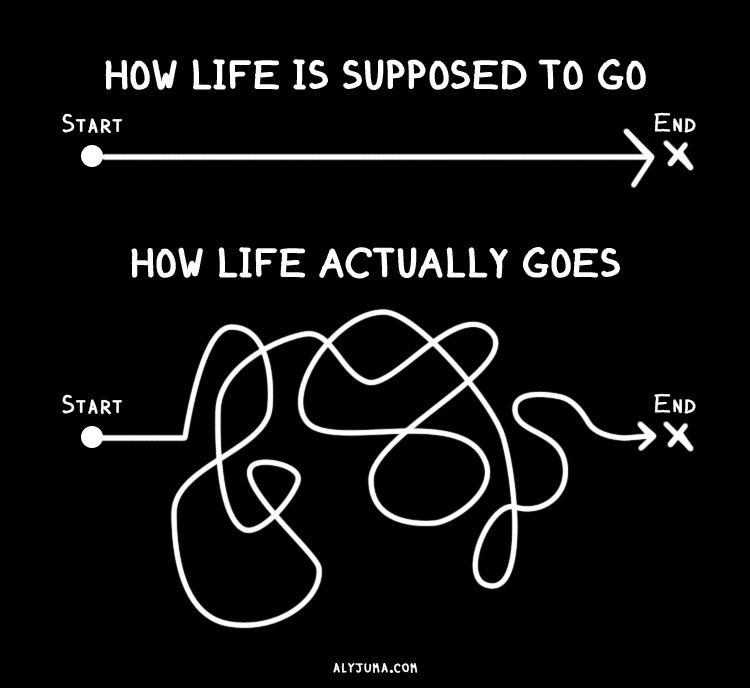
\includegraphics[height=0.9\textheight]{lifepath}
    Bild von \cite{lifepath-pic}
\end{frame}


\begin{frame}[c]{Planlosigkeit garantiert Scheitern}
    \begin{aquote}{Benjamin Franklin}
        If you fail to plan, you are planning to fail!
    \end{aquote}
\end{frame}

\begin{frame}[c]{Warum Planen}
    \large
    Man möchte Verstehen:
    \begin{itemize}[<+(1)->]
        % \item Versuch, das Ziel zu verstehen
        \item \textbf{Wann} das Ziel erfüllt ist
        \item \textbf{Was} der momentane Stand ist
        \item \textbf{Wie} das Ziel erreicht werden kann
        \item Welche \textbf{Hindernisse} auf dem Weg sind
        \item Was die \textbf{nächsten Schritte} sind
    \end{itemize}
    \pause
    Kurz: Die \textbf{Gesamtsituation}
\end{frame}


\subsection{Erfolg Definieren}
\pnote{Auf Ablauf eingehen}


\begin{frame}[c]{Problem: Ziel ist Unklar}
    \normalsize
    \includegraphics[width=\textwidth]{unclear-goals} \\
    How to wreck your finances. (Bild von \cite{unclear-goals-pic})
\end{frame}


\begin{frame}[c]% {Aufgabe: Klar definieren, wann das Ziel erreicht ist}
    % \begin{exampleblock}{Aufgabe}
    %     Definiere für jedes Ziel eindeutig, wann dieses Erreicht worden ist.
    % \end{exampleblock}
    % \begin{alertblock}{Aufgabe}
    %     Definiere für jedes Ziel eindeutig, wann dieses Erreicht worden ist.
    % \end{alertblock}
    \begin{block}{Aufgabe: Definiere Erfolg}
        Definiere für jedes deiner Ziele \textbf{eindeutig}, wann es erreicht wurde.
    \end{block}
    \pnote{Zeit: 5-10min}
\end{frame}

% We first need a clear-cut definition as to when the goal is achieved. You
% might have heard of ‘SMART’ goals before, Specific, Measurable, Achievable,
% Robust and Time-bound. I want you to focus on Specific and Measurable first,
% since they are good indicators of having achieved the goal. For each of your
% goals, be as specific as you realistically can about what you want. If
% possible, find something measurable.
%
% When trying to learn French, your Specific and Measurable goal might be to be
% capable of longer-duration interactions with native speakers, without a major
% stumble or needing to look up words; with the goal being achieved when you
% had five such 30min interactions. It does not need to be the full mastery of
% a language, ‘getting my driver’s license’ is a decent goal criterion for
% ‘learn to drive’.
%
% For all of your goals, clearly define when you have achieved them.
%
% Usually the best way is to ask how people who have achieved what you want to
% do knew that they have achieved it. You might want to do this later and adapt
% your own criteria based on their answers. While you’re at it, ask them about
% some tips for the way.


\subsection{Meilensteine}


\begin{frame}[c]{Problem: Abhängigkeiten}
    \normalsize
    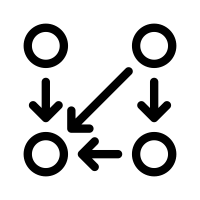
\includegraphics[height=0.9\textheight]{dependency}
    (Bild von \cite{dependency-pic})
\end{frame}



\begin{frame}[c]
    \begin{block}{Aufgabe: Definiere Meilensteine}
        Finde alle Meilensteine (\blue{Projekte}, nicht \green{Aufgaben}), die
        notwendig sind, um deine Ziele zu erreichen.
    \end{block}
    \pnote{Zeit: 5-10min}
\end{frame}


% Defining Sub-goals (5-10min)
% Bigger goals tend to have steps. They are not just done suddenly, there are
% steps in between that need to be achieved, sometimes in a specific order,
% before the actual goal can be achieved. When you want to do that awesome
% trip, you need to book the hotel beforehand, you need to check if you need to
% apply for visas, and buy new hiking shoes if you need some. These are all
% milestones, or sub-goals that are necessary to achieve the actual goal.
% Progress on one of them means progress towards your goal.
%
% While you can work independently on some (booking hotel and buying new gear),
% others, like checking if visas are required visas, might create additional
% milestones - getting the required visas.
%
% Sub-goals should be achievable within a few days at most. It’s okay if they
% only need a few minutes - as long as they are conceptually enclosed.
% (Sometimes there are sub-goals of sub-goals, that’s ok too!)
%
% Find and write down all relevant sub-goals for each of your bigger goals.


\subsection{Scheitern durch Erfolg}

\begin{frame}[c]{Problem: Gefühl von Fortschritt}
    \large
    \begin{aquote}{Charlie Munger, Berkshire Hathaway}
        Don’t just do something ... stand there
    \end{aquote}
    \normalsize
    Zu: Wie man nicht auf Aktienfluktuationen überreagiert.
    \pnote{Häufig fühlt es sich nur nach Fortschritt an}
\end{frame}


\begin{frame}[c]
    \vspace{1cm}
    \begin{block}{Aufgabe: Gefühlter Fortschritt}
        Versuche Situationen zu finden, die sich nach Fortschritt anfühlen
        könnten, aber nicht deinem Ziel näher kommen.
    \end{block}
    \vspace{0.5cm}
    \begin{block}{Aufgabe: Versuche zu Cheaten}
        Finde Möglichkeiten, den Weg zu deinem Ziel abzukürzen. Schreibe
        alles auf, was dir in den Sinn kommt. Nutze jede Abkürzung, die auch
        wirklich dein Ziel erreicht!
    \end{block}
    \pnote{Zeit: 15min}
    \pnote{Auch: Wie du dir selbst vorgaukeln könntest, es wäre Fortschritt ('es fühlt sich so an')}
\end{frame}


% Death by Winning (5min)
% Sometimes, it feels like we are working towards a goal and being successful,
% but we are actually not.
%
% There is a story of the early days of the X.com/PayPal rivalry. They were
% both frantically trying to put in more hours than the other and trying to get
% one more feature than the other. And for them it felt like progress. Except:
% It did not matter. Customers mostly ignored these features.
%
% If all you care about is to keep the ship’s nose pointed east, you won’t
% notice the ship sinking. Working for years on your career will only amount to
% so much if you realize that your (now broken) family would have been more
% important.
%
% There are situations in which we think everything is going fine, and we see
% progress happening towards a goal. Only to realize after weeks, months, or
% sometimes years, that while the ship’s nose was pointed east, the sails have
% never been set. The ship did not move forward - in fact, the waves slightly
% pushed it back.
%
% There would have been a simple way to avoid that - just the additional check
% that the sails are set. Just one small thing. If we just had made sure that
% the boat is actually moving, we could be much closer to our goal.
%
% By avoiding these kinds of situations, you can avoid wasting immense amounts
% of time, effort, and energy. Just staying clear of those will improve your
% effectiveness tremendously.
%
% Look for ways you might ‘cheat’ your goal, and write them down. If it is an
% actual shortcut, use it! If it will instead not get you closer to your actual
% goal, stay away from it.




\subsection{Leit- und Verzögerungsmaße}
% Leitmaß & Verzögerungsmaß


\begin{frame}[c]{Beispiel: Gewichtsreduktion}
    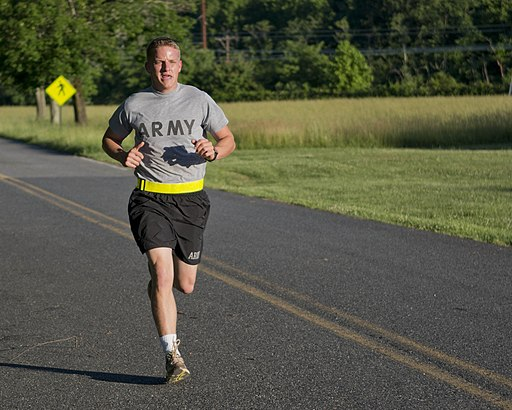
\includegraphics[height=0.8\textheight]{weight_loss} \\
    (Bild von \cite{weight-loss-pic})
    \pnote{Klassisches Neujahrsziel}
\end{frame}

\begin{frame}[c]{Definition: Verzögerungsmaß}
    \large
    \pause
    \textbf{Beispiel:} Gewicht
    \begin{itemize}[<+(1)->]
        \item Information über stand Jetzt oder Vergangenheit
        \item Was bereits passiert ist
        \item Einfach zu Erfassen
        \item Wird beeinflusst von vielen externen Faktoren
        \item Nützlich zu haben
        \item Aber kann nicht verändert werden
    \end{itemize}
    \pnote{Die meisten Wichtigen Dinge werden über Verzögerungsmaße gemessen}
    \pnote{Okay: Ziel Komplett erreicht (boolean)}
    \pnote{Muss nicht unbedingt 'graduell' sein}
\end{frame}


\begin{frame}[c]{Beispiel Gewicht: Einfluss Externer Faktoren}
    % trim = l b r t
    \small
    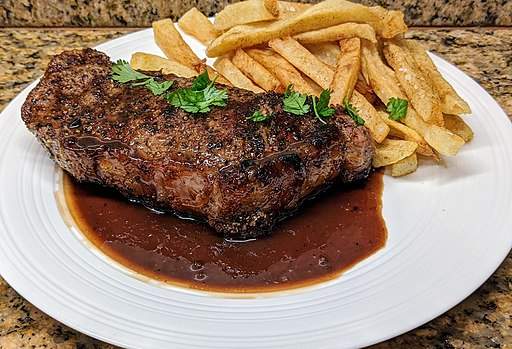
\includegraphics[width=0.7\textwidth, clip=true, trim = 15 150 15 20]{steak}
    (Bild von \cite{steak-pic})
    \large
    \begin{itemize}[<+(1)->]
        \item Getrunkenes Wasser
        \item Kohlenhydrate der letzten Tagen
        \item Verändert sich über den Tag
        \item Messung unter anderen Bedingungen
    \end{itemize}
\end{frame}

\begin{frame}[c]{Definition: Leitmaß}
    \large
    \pause
    \textbf{Beispiel:} Kaloriendefizit pro Tag
    \begin{itemize}[<+(1)->]
        \item Kann Erfolg Voraussagen
        \item Misst Aktionen, die Ergebnisse liefern
        \item Einfach zu Beeinflussen
        \item Häufig Schwer zu Messen
    \end{itemize}
    \pnote{Garantiert Ergebnisse}
    \pnote{Sollte graduell sein, muss es aber nicht}
    \pnote{Fokus sollte auf 'einfach messbar' sein}
\end{frame}


\begin{frame}[c]{Beispiel: Andrej Karpathy}
    \large
    Ziel: Defizit von ~500kcal pro Tag
    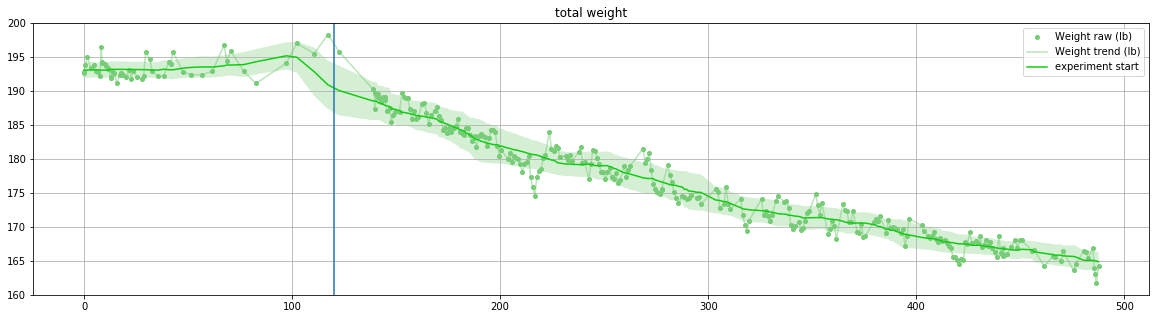
\includegraphics[width=\textwidth]{weight} \\
    (Bild von seinem Blog, \cite{weight-pic})
\end{frame}


% \begin{frame}[c]{Tipps für Leitmaße}
%     \large
%     \begin{itemize}[<+(1)->]
%         \item Bevorzuge robuste Maße (schwer zu Manipulieren)
%         \item Bevorzuge einfach Messbare Werte
%         \item Okay: Jeden Tag 30 minuten konzentriert Arbeiten
%     \end{itemize}
% \end{frame}


\begin{frame}[c]
    \begin{block}{Aufgabe: Definiere Leit- und Verzögerungsmaße}
        Versuche robuste Leit- und Verzögerungsmaße für jedes deiner Ziele zu
        Definieren.
    \end{block}
    \pnote{Zeit: 20min}
    \pnote{Verzögerungsmaß ist im zweifel einfach das Ziel selbst nach definierten Kriterien erreicht haben}
\end{frame}


% Exercises
% You get bonus points for robust Lead measures - if it’s hard for you to
% manipulate them, or cheat the measures in any way.
%
% For some goals (or even just some milestones) it is hard up to impossible to
% find good Lead measures - because circumstances, conditions and targets
% change so fast. You could meta-measure in these situations:
%
% Make one next action step towards the goal today, and make sure at least one
% is ready for tomorrow.
% I use similarly defined metrics for two of my goals.
%
% Go through your goals and Milestones and note which already have a Lag
% measure.
%
% Define Lead and Lag measures for each of your goals and milestones. If it
% seems impossible to find good Lead measures, set a timer to 3min and attempt
% to find one during this time.




% \begin{frame}[c]{Definition: Lag Measure}
%     \begin{itemize}[<+(1)->]
%         \item Information about the past
%         \item what already happened
%         \item easy to capture
%         \item It's useful to keep score
%         \item but it can't be changed
%     \end{itemize}
% \end{frame}
%
%
% \begin{frame}[c]{Definition: Lead Measure}
%     \begin{itemize}[<+(1)->]
%         \item Predict success
%         \item measure actions, that generate results
%         \item easy to influence
%         \item (sometimes) hard to capture
%     \end{itemize}
% \end{frame}


% We first take a good look at what Lead and Lag measures are before using them
% to make our goals and milestones more tangible.
%
% The fallacy of Lag measures
% A classical new-years goal is to lose weight. Let’s say the goal is to lose
% 10 kg until next year. At first, losing weight is rapid and easy. Until
% suddenly, you gain a bit. But then you lose weight again. And the reverse
% again. Your actual weight is fluctuating a lot, and it does not really feel
% like progress at all. This goes on for a bit, until most people quit.
%
% When trying to lose weight, weight is the thing you want to get down
% long-term. But there are a lot of factors influencing weight in the
% short-term. These include factors such as the time of day when measuring, how
% much water you just drank, the percentage of carbohydrates in last weeks’
% diet, and so much more. All of them can influence your weight right now
% tremendously. Noticing actual trends is hard, and impossible with less than
% two weeks of data. Most quit before a trend can manifest - but they couldn’t
% see a trend in the first place, since they don’t remember last week’s exact
% measure.
%
% Weight, just like most interesting metrics, is a Lag measure. While it is
% your ultimate goal, it is very susceptible to a wide range of factors and
% thus quite volatile in the short term. It is only useful in averages and
% long-term-trends. Results lag behind if you will. Looking at it today and
% feeling depressed about it will not do you any good - and it will not get you
% closer to your goal, either. So what if you want to measure something to feel
% good about it?
%
% Lead measures
% What you could measure instead, is daily calorie intake. Not just the intake,
% but ensuring that you have a certain calorie deficit each day. With a daily
% deficit of 500kcal, you are short 3500kcal every week, which is the energy
% stored in roughly 500g fat. The biggest benefit: it’s something that can be
% done every day, and it’s not susceptible to short-term variance. Keeping this
% up for Half a year will make you weigh less about 13.5 kg - a third more than
% the initial years’ goal of 10 kg.
%
% Daily calorie deficit is a Lead measure. Lead measures have much shorter
% intervals, such as days or weeks, and lead to the goal - eventually. For
% these, consistency is key. Consistently hitting your lead measures ensures
% that you hit your lag measures as well.
%
% Tips for applying them
% A Lag measures can be singular as well: ‘Finish writing the Goal Setting
% Workshop post’ is a current Lag measure for a milestone of mine. It does not
% necessarily have to be clear how lag measures are achieved, but it should be
% clear how to hit the lead measures.
%
% Lead measures might change across milestones, the important part is having a
% Lead measure for each milestone.
%
% It is absolutely okay for both Lead and Lag measures to be time-bound: One of
% my Lead measures is to read 30min in a focused manner each day. Sometimes I
% read up to two hours, but 30min is the minimum. No average, no ‘but I did
% double yesterday’, 30min a day, every day. This takes away the pressure to
% achieve a bit. This is especially useful when it is hard to estimate workload
% - I just cannot estimate the time required for reading a chapter or even a
%   single page, since both chapters and pages are sometimes more, and
%   sometimes less dense with information. Making it time-bound increases
%   predictability as well: you’re done after 30min, continue tomorrow - though
%   of course, there’s nothing stopping you from doing more work either, and
%   doing so feels incredibly good.
%
% Exercises
% You get bonus points for robust Lead measures - if it’s hard for you to
% manipulate them, or cheat the measures in any way.
%
% For some goals (or even just some milestones) it is hard up to impossible to
% find good Lead measures - because circumstances, conditions and targets
% change so fast. You could meta-measure in these situations:
%
% Make one next action step towards the goal today, and make sure at least one
% is ready for tomorrow.
% I use similarly defined metrics for two of my goals.
%
% Go through your goals and Milestones and note which already have a Lag
% measure.
%
% Define Lead and Lag measures for each of your goals and milestones. If it
% seems impossible to find good Lead measures, set a timer to 3min and attempt
% to find one during this time.


\subsection{Nächste Schritte}


\begin{frame}[c]{Problem: Ungewissheit}
    \large
    \begin{aquote}{Cassandra Clare}
        One must look at the next step on the path ahead, rather than the
        mountain in the distance, or one would never reach one's goal.
    \end{aquote}
\end{frame}


\begin{frame}[c]
    \begin{block}{Aufgabe: Finde die Nächsten Schritte}
        Finde die drei \green{Aufgaben} für jeden Meilenstein, die nicht lang
        dauern, und du direkt tun könntest. Erledige:
        \begin{itemize}
            \item die erste Aufgabe jetzt
            \item die zweite Aufgabe morgen vor 11 Uhr früh
            \item die dritte Aufgabe vor 11 Uhr früh übermorgen
        \end{itemize}
    \end{block}
    \pnote{Zeit: 10min}
\end{frame}


% Identify Next Actions (10min)
% At every point along the way, it is extremely important to have specific next
% actions. Sometimes the only things getting you closer to your goal are
% actions. Execution will focus on that more, but here is the basic idea: When
% in a situation where you could easily make progress towards your goals, you
% will not do so if you are unaware of the possibility.
%
% A next action is a clearly defined and described physical action that can be
% done immediately (if not blocked) and will bring you closer to one of your
% goals or milestones. Sometimes next actions are blocked, since you are
% waiting for a mail first, or need someone else to help you - be aware of
% those blockers.
%
% If you want to build an awesome tree house, and you go to the hardware store
% (getting color to paint a room), it can help to know if you need nails or
% not. If you noticed a week later, you would need more energy and momentum to
% go to the hardware store again. Knowing things like that at the right time
% will save a lot of energy and effort.
%
% Everything requiring more than two next actions to get it done is a project.
% Goals and milestones are necessarily projects, but you might be working on
% projects that are not part of your primary goals as well. Organizing a
% birthday party is unlikely part of your goals, but nonetheless something you
% might have committed to doing.
%
% For each of your milestones, find three next actions you could work on right
% now, each taking a few minutes at most.
%
% Do the first now (or later, but today)! Do the next tomorrow before 11am (or
% no later than 4h after waking up, whichever comes first), and the third the
% day after tomorrow before 11am. Ensure that you have new next actions to work
% towards by then.
%
% Take a break before continuing with Execution. Skip to conclusions if you
% have an execution system like gtd already.

\fpause

\section{Ausführung}

\subsection{Einführung}

\begin{frame}[c]{Problem: Ausführung}
    \large
    \begin{aquote}{Chris Sacca (Shark Tank)}
        Ideas are cheap. It's all about execution.
    \end{aquote}
    \pnote{Gibt grundsätzlich Zwei Perspektiven zur Ausführung}
\end{frame}


\begin{frame}[c]{Perspektive: Kurzfristig}
    \large
    \begin{itemize}
        \item Pomodoro
        \item Time-Blocking
        \item Arbeitszyklen
        \item Kaffee/Koffein
        \item Co-Working-Räume
        \item \enquote{Einfach machen}
    \end{itemize}
\end{frame}


\addtocounter{framenumber}{1}
\begin{frame}[standout]
    \Large
    Jetzt: Langfristig
\end{frame}

% > Ideas are cheap. It’s all about execution. - Chris Sacca (Shark Tank)
%
% While we already defined the first three next action items for each of your
% goals, they should be done the day after tomorrow. What then?
%
% There are two parts to execution, and they answer different timeframes to the
% questions ‘what do I do next?’.
%
% First is how to execute in the moment: While just sitting down and working on
% it is pretty effective, there are some techniques you might at least want to
% try, which could spice things up a bit. But just working and working and
% working on something is not guaranteed to work out. Being busy is absolutely
% not the same as being effective. Keeping the ships nose pointed east is fine,
% but you need to make sure that it’s moving as well.
%
% Second is the bigger-picture planning and execution. This includes taking a
% look at all the projects you want to work on, the tasks you have left, your
% progress and your current results, to determine if you’re going the right
% way. To determine that the ship is actually moving forward while pointed
% east. We’re primarily going to take a look at that one.
%
% We will take a look as to why execution tends to fail in the first place, to
% understand why an execution system is a decent approach to addressing these
% issues properly.


\subsection{Häufige Probleme}

\begin{frame}[c]{Häufige Probleme}
    % \large
    \footnotesize
    \begin{itemize}[<+(1)->]
        \item Aversion: Es ist unangenehm, über das Ziel oder die Ausführungspläne nachzudenken (Stress, Selbstschuld, Angst)
        % \item Aversion: When thinking about our goals or execution plans, we experience some form of discomfort (stress, guilt, dread)
        \item Ablenkung: Wir suchen andere angenehme Dinge, um uns abzulenken und prokrastinieren
        % \item Distraction: Instead of doing the hard work, we procrastinate and distract ourselves with urgent or pleasurable things instead
        % \item Zu wenig Motivation: Unser Ziel und unsere Pläne geben uns nicht mehr genug Energie
        % \item Limited motivation: Somehow our goal and our plans don’t give us energy any more
        \item Zu wenig Zeit: Wir sind mit etwas anderem beschäftigt
        % \item Limited time: It’s easy to be busy in the moment and focus on other things instead
        \item Zu wenig Energie: Wir sind zu müde, nach der Arbeit noch etwas weiteres zu tun
        % \item Limited energy: We are too tired to work on something else after a long day at work
        \item Zu wenig Aufmerksamkeit: Es ist nicht wirklich klar, was der nächste Schritt ist
        % \item Limited attention: It’s not even clear what we want to do, since it’s hard to keep track of everything
        \item Zu wenig Verantwortung: Es ist selten, dass jemand von uns erwartet, dass es fertig wird
        % \item Limited accountability: We rarely have someone else holding us accountable, resulting in conscious and unconscious guilt to increase accountability.
        \item Zu wenig Selbstvertrauen: Niedrige Selbstwirksamkeit ist eine sich selbst erfüllende Prophezeiung; Wir erwarten nicht, das Projekt abzuschließen
        % \item Limited self trust: A low self-efficacy self-fulfilling prophecy; We don’t think we will ultimately follow through, so we won’t
    \end{itemize}
\end{frame}


\begin{frame}[c]
    \begin{block}{Aufgabe: Grund für Misserfolg finden}
        Finde heraus, weswegen dein letztes größeres Projekt gescheitert ist,
        und was du diesmal anders machen könntest.
    \end{block}
    \pnote{5min}
\end{frame}


\begin{frame}[c]{Optional: Murphyjitsu}
    \large
    \begin{enumerate}[<+(1)->]
        \item Mache einen Plan.
        \item Stell dir vor, der Plan ist gescheitert.
        \item Wenn du überrascht von der Vorstellung bist, bist du fertig.
        \item Andernfalls, simuliere den wahrscheinlichsten Fehlermodus. Unternehme etwas dagegen. Wiederhole ab Schritt 2.
    \end{enumerate}
    \pause
    \tiny
    Mehr Informationen: \url{https://www.lesswrong.com/posts/N47M3JiHveHfwdbFg/hammertime-day-10-murphyjitsu}
\end{frame}


\begin{frame}[c]
    \begin{block}{Aufgabe: Murphyjitsu}
        Finde heraus, weswegen deine Ziele scheitern könnten, und unternehme
        etwas gegen wahrscheinliche Blockaden.
    \end{block}
    \pnote{Zeit: 20min}
\end{frame}


% Failing Execution (5min)
% Execution tends to regularly fail, and there is a number of reasons why.
% Taking some time to think about root causes, you might end up with a list
% similar to this:
%
% - Aversion: When thinking about our goals or execution plans, we experience some form of discomfort (stress, guilt, dread)
% - Distraction: Instead of doing the hard work, we procrastinate and distract ourselves with urgent or pleasurable things instead
% - Limited motivation: Somehow our goal and our plans don’t give us energy any more
% - Limited time: It’s easy to be busy in the moment and focus on other things instead
% - Limited energy: We are too tired to work on something else after a long day at work
% - Limited attention: It’s not even clear what we want to do, since it’s hard to keep track of everything
% - Limited accountability: We rarely have someone else holding us accountable, resulting in conscious and unconscious guilt to increase accountability.
% - Limited self trust: A low self-efficacy self-fulfilling prophecy; We don’t think we will ultimately follow through, so we won’t
%
% In fact, it might not be just one, it might be multiple reasons at once. And
% sometimes, that’s fine - as long as you don’t beat yourself up over it.
%
% There are ways to improve in-the-moment effectiveness, but they are band-aid
% at best and don’t help if you can’t get started in the first place. Execution
% systems go for multiple of these potential failure modes at once, helping us
% tremendously in achieving our goals.
%
% Figure out the main reasons why your last project or goal was unsuccessful,
% and what you would change next time.


\subsection{Verantwortungspartner}

% Forschung: 149/267 Teilnehmer
% Zufällig gruppe zugewiesen
% - gruppe 1 hat sich über die Ziele gedanken gemacht
%   rate that goal on the following dimensions: Difficulty, Importance, the
%   extent to which they had the Skills & Resources to accomplish the goal,
%   their Commitment and Motivation to the goal, whether or not they had
%   Pursued this goal before and if so their Prior Success.
% jede gruppe hat auch das getan, was die gruppe davor getan hat
% - Participants in Groups 2-5 were asked to write (type into the online survey)
% their goals and then to rate their goals on the same dimensions.
% - Group 3 was also asked to formulate action commitments.
% - Group 4 was asked to formulate action commitments and send their goals and
% action commitments to a supportive friend.
% - Group 5 was asked to formulate action commitments and send their goals,
% action commitments and weekly progress reports to a supportive friend.

\begin{frame}[c]{Fortschrittsberichte}
    \small
    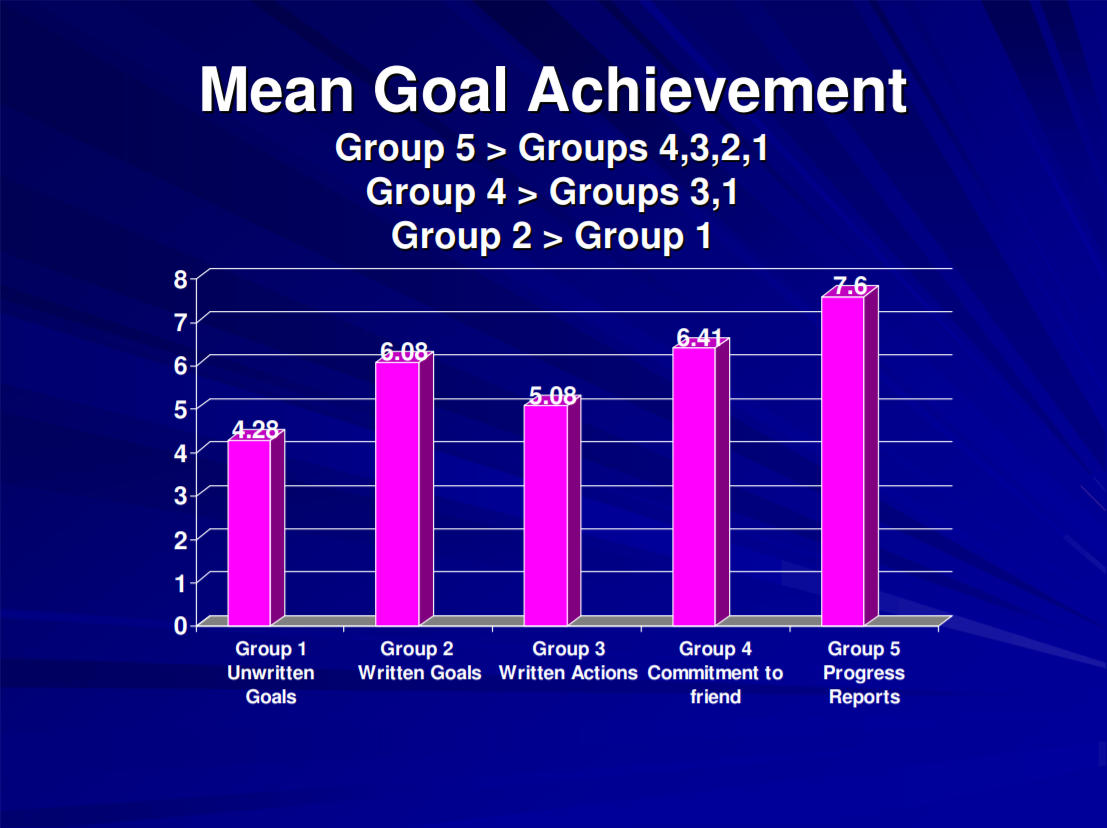
\includegraphics[height=0.8\textheight]{goal_achievement_all} \\
    Regelmäßige Fortschrittsberichte haben den höchsten Erfolg \cite{better-goals-2}.
    \pnote{Jede Gruppe auch immer das von den vorigen}
    \pnote{Gruppe 1: Gedanken gemacht über Schwere, Wichtigkeit, Fähigkeiten, Motivation, etc}
    \pnote{Gruppe 2: Aufschreiben}
    \pnote{Gruppe 3: 'Formulate Action Commitments'}
    \pnote{Gruppe 4: Send goals and action commitments to friend}
    \pnote{Gruppe 5: Send weekly progress reports to supportive friend}
\end{frame}


\begin{frame}[c]{Interaktion mit Verantwortungspartner}
    \begin{enumerate}[<+(1)->]
        \item Finde jemanden, mit dem du dich regelmäßig verabreden kannst
        \item Berichte von deinem Fortschritt seit dem letzten Treffen
        \item Gebe an, was deine nächsten Schritte sind, und was du bis zum nächsten Treffen erreichen möchtest
        \item Vereinbare den nächsten Termin
        \item Beim nächsten Treffen: Starte ab dem zweiten Schritt
    \end{enumerate}
    \pnote{Wichtig: Nicht Ziele 'Bewerten' lassen, gibt Studien, dass Erfolg reduziert}
\end{frame}


\begin{frame}[c]
    \begin{block}{Aufgabe: Finde einen Verantwortungspartner}
        Finde jemanden, mit dem du dich regelmäßig über deinen
        Fortschritt austauschen kannst, und vereinbare den ersten Termin.
    \end{block}
    \pnote{Zeit: 10min}
\end{frame}

% Accountability Partners (10min)
% One very simple way that will help you to get started and to keep doing it,
% is to have someone hold you accountable for it. In fact, it is a very simple
% execution system and will help a lot with the common failure modes.
%
% It mostly does not matter who will hold you accountable, but a friend who
% needs someone to hold them accountable for something themselves is ideal.
% Just schedule a meeting or call every week, month, or other timeframe you are
% comfortable with, and you’re good to go.
%
% The goal is that you state your goals and the progress you want to make each
% meeting and get asked about the progress you actually achieved prior to
% planning your progress the next meeting. That’s it. Repeat.
%
% Here are the steps again:
%
% - Find a friend to hold you accountable and schedule regular calls or meetings
% - Report progress and current challenges on your goal(s)
% - State your next steps and what you want to achieve until next time (Lead measures!)
% - Schedule the next call/meeting before hanging up/separating
% - Repeat from Step 2 at the next call/meeting
%
% Obviously you shouldn’t talk the entire time. Intersperse your meeting with
% listening to the progress and next steps of your friend. I’m doing my monthly
% planning similarly with a friend, and it helped me tremendously to stay
% focused and to achieve more. In our experience, talking about
% non-goal-related topics in the first few minutes is a good and comfortable
% way to start.
%
% Find yourself an accountability partner and schedule the first meeting.
%
% You might want to take a look at Execution Systems before actually doing so.
% It explains a similar system that is synergistic with Accountability
% Partners, if implemented right.





% \subsection{Selbstmanagementsysteme}


% Setting up an Execution System (30min)
% Accountability Partners is in itself a basic Execution System, and works best
% when implemented with a second Execution System over a different timeframe.
%
% Fundamentally, every execution system has these four parts, weighed as required:
%
% Review: Taking a look at the progress that happened, evaluating taken approaches
% Retrospective: Taking a look at the current process, making adjustments for parts that are not working as well as they should
% Planning: Planning milestones and tasks for the next timeframe until Review, clarifying when they are done
% Execution: Actually working on the collected Tasks, in a way to make progress on them.
% Another very important parameter is your cycle frequency, or how long it takes for a full cycle in your Execution System. We’ll take a look at each of these parts in detail, before we discuss how to implement it.
%
% Review
% A regular review is the single most important part in an execution system. It
% enables both planning and execution to build on the most recent insights of
% how things stand.
%
% The goal is to get a bigger-picture perspective about the goals you are
% working on. The most important part is reviewing what was planned and what
% was achieved, and just generally taking inventory of made progress. If you
% haven’t marked some tasks as done yet, now is the time to bring your notes up
% to date.
%
% A big focus is how you approach the problems you encounter and how well your
% approaches are working. If they’re not working well, you adjust them during
% ‘Retrospective’, to do better next cycle.
%
% When collecting decent Lead/Lag metrics, plotting them can be really useful
% in noticing outliers and general trends. It is also motivating to see the
% progress that has been made, making it easier to keep going.
%
% Retrospective
% This is the phase to make changes to your execution system and how to use it,
% to adapt it to your needs. Beware of many changes at once, since a single
% change can modify the nature of Execution Systems tremendously. It’s not
% necessary to make changes all the time, but if there’s something bugging you,
% figure out a way to improve it. Even small changes can help you substantially
% - especially in the long run.
%
% This is also the time to figure out solutions for obstacles preventing you to
% execute during ‘Execution’ - e.g. getting a ‘Do not disturb’-sign to tell
% your flatmates when you prefer not to get interrupted.
%
% If you noticed that a Lead or Lag measure does not fit for the goal or
% milestone, now is the time to make adjustments.
%
% Planning
% This is more or less a ‘mini’-planning section, with the core focus being to
% ensure you have at least one if not multiple next actions for each goal and
% project.
%
% After reviewing the progress and status for all of your projects and goals,
% you might need to plan or adapt the next steps for each. It might not be
% necessary, but more often than not I notice a missing task, clarify
% descriptions or reorganize priorities.
%
% Execution
% When actually working on tasks, it can be helpful to try one of the following
% productivity helpers:
%
% Pomodoro
% Work Cycles
% Co-Working Spaces
% A ‘Pomodoro’ is a 30-min interval with 25min work-time and a break of 5min.
% Work Cycles are similar, with 30min work time interspersed with 10min breaks,
% in which you do a bit of work-related planning and reviewing.
%
% Co-Working spaces such as libraries are great, many have found themselves to
% be much more productive there. It’s harder to let yourself slack off, and
% easier to stay productive, with or without pomodoro. A virtual co-working
% space such as the LessWrong study hall can have the same effects.
%
% However, it’s all about actually getting your next action items done, and
% making progress on your goals, projects and milestones. So feel free to use
% whatever method best works for you.
%
% Timeframe
% The timeframe you plan for is an important factor. It can be anything you are
% comfortable with, but I would recommend a one-week-cycle as a basis with a
% complementary one-month-cycle of Accountability Partners. But a weekly cycle
% is essential to enable continuous execution of your goals.
%
% Putting Everything Together
% Your execution system should enable you to easily figure out what you both
% want and need to do in the moment. New tasks get added during the weekly
% review/planning session as well as when something comes up during the week.
%
% The core parts to enable that is the weekly review - it is normal to forget
% details during the week. I tend to have both completed tasks not yet marked
% as done as well as new open tasks not yet included, but maybe written down
% somewhere else. The weekly review is the time to synchronize the execution
% system to what happened in the real world.
%
% As long as your execution system is (mostly) current when taking a look at it
% during the week, you are able to get the open tasks that require your
% attention now.
\fpause
 % could use expansion
\section{Conclusion}


\begin{frame}[c]{Conclusion Regarding the Integration of RUST}
    \begin{itemize}[<+(1)->]
        \item Test the alternatives more
        \item Better integration should be possible
        \item All in all: Went better than expected
    \end{itemize}
\end{frame}


\begin{frame}[c]{Conclusion Regarding Computation Comparisons}
    \begin{itemize}[<+(1)->]
        \item Reduction of memory usage during correction achieved
        \item Reduction of runtime achieved
        \item Parallelism does not offer significant benefits yet
    \end{itemize}
\end{frame}


\begin{frame}[c]{Remaining Questions}
    \begin{itemize}[<+(1)->]
        \item Writing code for faster parallelism
        \item Speedup when parallelizing more
        \item Pure implementations needing even less memory?
        \item Is KR faster for bigger matrices?
    \end{itemize}
\end{frame}



 % finished?
% \section{Section}

\subsection{Subsection one}
\subsection{Subsection two}


\section{Examples}

\begin{frame}[c]
     Here a citation: \cite{benchcpp}
\end{frame}


\begin{frame}[c]{Example slide}
    \pnote{The items to discuss are:
    - First Element \n
    - Second Element
    Later on, also:
    - Third Element
    }
    \pnote{Note in next line}
    \Large
    \begin{itemize}[<+->]
        \item Shows immediately!
        \item Second Element
        \item Third Element
    \end{itemize}
\end{frame}


\begin{frame}[c]{Element visible in handout only}
    \Large
    \begin{itemize}[<+(1)->]
        \item Delay of one slide!
        \item Second Element
        \item<handout> Only visible in Handout!
    \end{itemize}
    \pnote{The notes are visible BEFORE the slide in pdfpc!}
\end{frame}


\begin{frame}<handout:0>[c]{Not Visible in Handout}
    \Large
    \begin{itemize}[<+(1)->]
        \item These slides do not show in Handout
        \item Second Element
        \item Third Element
    \end{itemize}
\end{frame}


\begin{frame}[c]{Prevent Wobbeling}

    Simply use an overlayarea!

    % \begin{verbatim}
    %     \begin{overlayarea}{\textwidth}{0.8\textheight}
    %     \end{overlayarea}
    % \end{verbatim}

\end{frame}

% '\include'
% - gives speed bonus when building, through caching in a seperate *.aux file
% - has a 'page break'
% - cannot be nested
% ------------- VS -------------
% '\input'
% - can be nested
% - does not have 'page breaks'
% - gives no caching benefit


%%%%%%%%%%%%%%%%%%%%%%%%%%%%%%%%%%%%%%%%%%%%%%%%%%%%%%%%%%%%%%%%%%%%%%%%%%%%%%%%%%%%%%%%%%%%%%%%%%%



%%%%%%%%%%%%%%%%%%%%%%%%%%%%%%%%%%%%%%%%%%%%%%%%%%SOURCES%%%%%%%%%%%%%%%%%%%%%%%%%%%%%%%%%%%%%%%%%%
\section{Quellen}
\begin{frame}[c,fragile,allowframebreaks]{Quellen}
% \bibliographystyle{plainnat}
\bibliographystyle{ieeetr}
\bibliography{references.bib}
\end{frame}


\appendix
\backupbegin

\begin{frame}[c]{Rust: Code Example}
    \begin{codeboxed}{Code Example 1}
    \inputminted[linenos, fontsize=\normalsize]{Rust}{code/code_ownership.rs}
    \end{codeboxed}
\end{frame}

\begin{frame}[c]{Rust: Code Example}
    \begin{codeboxed}{Output Nr. 1}
        \footnotesize
        \verbatiminput{code/output1.txt}
    \end{codeboxed}
\end{frame}

\begin{frame}[c]{Rust: Code Example}
    \begin{codeboxed}{Code Example 2}
    \inputminted[linenos, fontsize=\normalsize]{Rust}{code/code_ownership2.rs}
    \end{codeboxed}
\end{frame}

\begin{frame}[c]{Rust: Code Example}
    \begin{codeboxed}{Output Nr. 2}
        \footnotesize
        \verbatiminput{code/output2.txt}
    \end{codeboxed}
\end{frame}

\backupend


\end{document}
